\documentclass{article}

\usepackage[english]{babel}
\usepackage[utf8x]{inputenc}
\usepackage{chemfig}
\usepackage[version=3]{mhchem}
\usepackage{listings}
\usepackage{graphicx}
\usepackage{enumitem}

\begin{document}

\title{\textbf{Schema.org Injector} \\ \emph{Dokumentation} }
\author{Stefan Haberl, Mathias Meinschad \\ \emph{STI Informatik}}
\date{February 13, 2017 \\ 
\includegraphics[width=0.25\textwidth, height=0.25\textwidth]{icon.png}}


\maketitle
\newpage


\tableofcontents
\newpage


% % % % % % % % % % % % %
% PROJECT
% % % % % % % % % % % % %
\section{Project}
\subsection{Overview}
Our goal for this project was to develope an extension for the CMS-system \textbf{TYPO3}, which allows the users to inject schema.org annotations inside their webpages.

Each page can be associated with JSON-LD files, which then are injected into the pages \textbf{head tag}.

\subsubsection{Specifications}
	\begin{itemize}
		\item Inject JSON-LD into single page
		\item Inject JSON-LD into multiple pages
		\item Easy to set up and intuitive customizations
		\item Compatibility to as many TYPO3 versions as possible
	\end{itemize}


\subsection{JSON-LD}
JSON-LD is a method of encoding Linked Data. It is build up onto of the most common data format used for asynchronous browser/server communication: \textbf{JSON}. As you can see in the example below, JSON-LD just extends JSON with some key words. We will explain some of these later in this documentation.

\subsubsection{Why JSON-LD?}
\begin{itemize}
	\item easy readable for humans and machines
	\item standard libraries for nearly any programming language
	\item HTML is not required, like in other schema mark-up methods (RDFa or microdata)
\end{itemize}

\subsubsection{Example of JSON-LD}
Here you can see a minimal example of JSON-LD:
\begin{lstlisting}
	<script type="application/ld+json">
	{
	  "@context": "http://schema.org/",
	  "@type": "Person",
	  "name": "Albert Einstein"
	}
	</script>
\end{lstlisting}
Those keys with an \textbf{@} in front are JSON-LD specific keywords. \emph{@context} is needed for specifying the keys. It tells the application how to interpret the rest of the data. Furthermore it also know what type of data has to be associated with the specific keys.
	


\subsection{Typo3 CMS}
\subsubsection{Overview}
\begin{itemize}
	\item Typo3 is an open source Content Managment System
	\item developed by: Kasper Skårhøj
	\item released: 1998
	\item current version: 8.5.1 (January 25, 2017)
	\item languages: PHP, SQL und JavaScript
	\item Building page with TypoScript and Fluid
\end{itemize}


% % % % % % % % % % % % %
% OUR EXTENSION
% % % % % % % % % % % % %
\section{Our Extension and how it works}
\subsection{General}
\begin{itemize}
	\item TYPO3 uses extension keys to allow unique identifying each extension
	\item extension key registered:  \textbf{schema\textunderscore injector}
	\item Developed with JetBrains PhpStorm
	\item XAMPP for local testing
	\item Will be published in TEM (Typo3 Extension Repository)
\end{itemize}
	
\subsection{Technical}
\begin{itemize}
	\item using hooks to manipulated rendered data
	\item persist settings into database
	\item use page ID to check if an injection is configured for a specific page
\end{itemize}


\subsection{How it works}
\begin{figure}[ht]
	\centering
	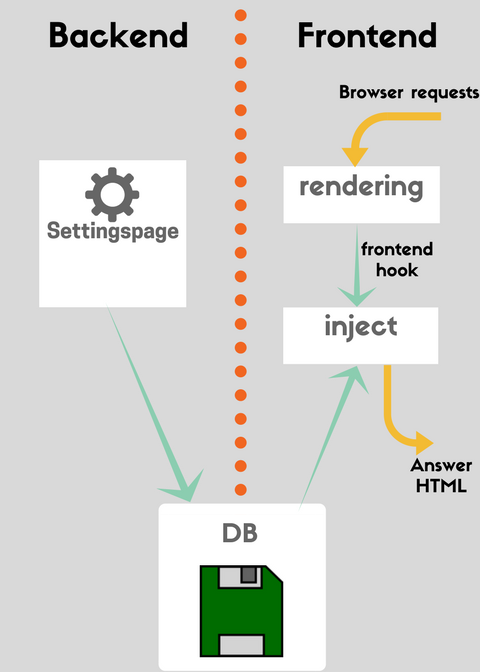
\includegraphics[height=0.75\textwidth]{work_flow.png}
	\caption{This illustration describes how our extension works in Typo3.}
	\label{work_flow}
\end{figure}
As you can see in figure \ref{work_flow} we built a backend and a frontend module.

The backend module displays the interface and is used to upload JSON-LD files to the server.
Furthermore it is needed to inject Typo3 pages with uploaded JSON-LD files and to delete injections from the pages.

The frontend module is handling the technical injections and rendering of the HTML pages.
Therefore we place a <script> tag in the HTML header. Where we just copy the whole JSON-LD file into this tag.



% % % % % % % % % % % % %
% Interface
% % % % % % % % % % % % %
\section{Interface}
\begin{figure}[ht]
	\centering
	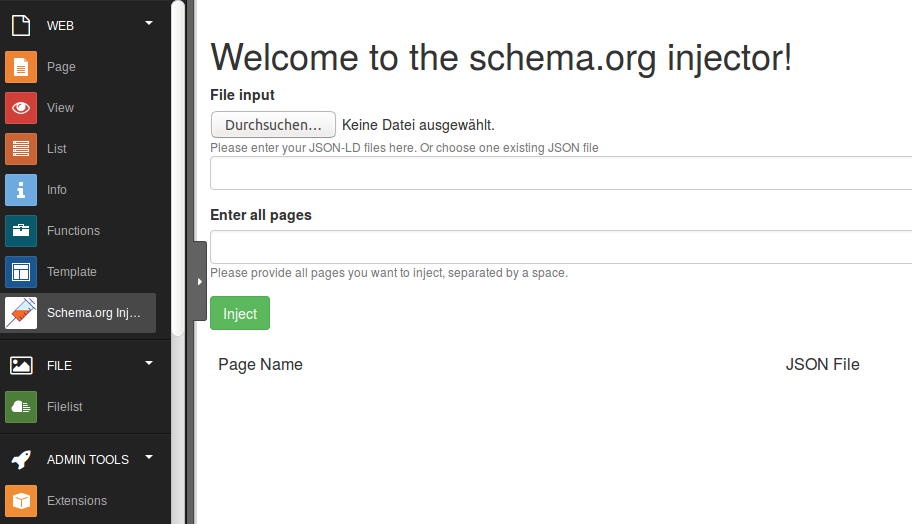
\includegraphics[width=1.0\textwidth]{backend_module.png}
	\caption{This is an image of the interface of our extension.}
	\label{interface}
\end{figure}

As you can see in the figure \ref{interface} our extension is very intuitive and simple. On the top of the interface is a file uploader. The extension user can upload his/her JSON-LD files onto server. We did not made any specific validation tests. It just will be checked if it is a JSON-LD file. The responsibility of a correct JSON-LD file relies on the user.

Below the file uploader it is possible to select an already uploaded JSON-LD file. This field is necessary because the extension do not allow two files with same name.

Further down the page input field is placed. The user has to name all the pages, where the uploaded or selected JSON-LD file should be injected. As a comfort feature the extension allows a wildcard \textbf{\%}.

This section could be easily improved with check boxes of all active pages in Typo3. So the user just has to check all pages where the injection should happen.


% % % % % % % % % % % % %
% OUR PROBLEMS
% % % % % % % % % % % % %
\section{Our Problems}
\begin{itemize}
	\item No experience with Typo3
	\item Caching behaviour in Typo3 while development (can't be completely turned off)
	\item Documentation is often out of date
	\item Small community, nearly no forums
	\item Low basic knowledge in PHP
	\item Solutions for older version not suitable for us
	\item Typo3 in general: TypoScript, how to inject code \dots
\end{itemize}

\end{document}